% Options for packages loaded elsewhere
\PassOptionsToPackage{unicode}{hyperref}
\PassOptionsToPackage{hyphens}{url}
\PassOptionsToPackage{dvipsnames,svgnames,x11names}{xcolor}
%
\documentclass[
  letterpaper,
  DIV=11,
  numbers=noendperiod]{scrartcl}

\usepackage{amsmath,amssymb}
\usepackage{iftex}
\ifPDFTeX
  \usepackage[T1]{fontenc}
  \usepackage[utf8]{inputenc}
  \usepackage{textcomp} % provide euro and other symbols
\else % if luatex or xetex
  \usepackage{unicode-math}
  \defaultfontfeatures{Scale=MatchLowercase}
  \defaultfontfeatures[\rmfamily]{Ligatures=TeX,Scale=1}
\fi
\usepackage{lmodern}
\ifPDFTeX\else  
    % xetex/luatex font selection
\fi
% Use upquote if available, for straight quotes in verbatim environments
\IfFileExists{upquote.sty}{\usepackage{upquote}}{}
\IfFileExists{microtype.sty}{% use microtype if available
  \usepackage[]{microtype}
  \UseMicrotypeSet[protrusion]{basicmath} % disable protrusion for tt fonts
}{}
\makeatletter
\@ifundefined{KOMAClassName}{% if non-KOMA class
  \IfFileExists{parskip.sty}{%
    \usepackage{parskip}
  }{% else
    \setlength{\parindent}{0pt}
    \setlength{\parskip}{6pt plus 2pt minus 1pt}}
}{% if KOMA class
  \KOMAoptions{parskip=half}}
\makeatother
\usepackage{xcolor}
\setlength{\emergencystretch}{3em} % prevent overfull lines
\setcounter{secnumdepth}{-\maxdimen} % remove section numbering
% Make \paragraph and \subparagraph free-standing
\ifx\paragraph\undefined\else
  \let\oldparagraph\paragraph
  \renewcommand{\paragraph}[1]{\oldparagraph{#1}\mbox{}}
\fi
\ifx\subparagraph\undefined\else
  \let\oldsubparagraph\subparagraph
  \renewcommand{\subparagraph}[1]{\oldsubparagraph{#1}\mbox{}}
\fi

\usepackage{color}
\usepackage{fancyvrb}
\newcommand{\VerbBar}{|}
\newcommand{\VERB}{\Verb[commandchars=\\\{\}]}
\DefineVerbatimEnvironment{Highlighting}{Verbatim}{commandchars=\\\{\}}
% Add ',fontsize=\small' for more characters per line
\usepackage{framed}
\definecolor{shadecolor}{RGB}{241,243,245}
\newenvironment{Shaded}{\begin{snugshade}}{\end{snugshade}}
\newcommand{\AlertTok}[1]{\textcolor[rgb]{0.68,0.00,0.00}{#1}}
\newcommand{\AnnotationTok}[1]{\textcolor[rgb]{0.37,0.37,0.37}{#1}}
\newcommand{\AttributeTok}[1]{\textcolor[rgb]{0.40,0.45,0.13}{#1}}
\newcommand{\BaseNTok}[1]{\textcolor[rgb]{0.68,0.00,0.00}{#1}}
\newcommand{\BuiltInTok}[1]{\textcolor[rgb]{0.00,0.23,0.31}{#1}}
\newcommand{\CharTok}[1]{\textcolor[rgb]{0.13,0.47,0.30}{#1}}
\newcommand{\CommentTok}[1]{\textcolor[rgb]{0.37,0.37,0.37}{#1}}
\newcommand{\CommentVarTok}[1]{\textcolor[rgb]{0.37,0.37,0.37}{\textit{#1}}}
\newcommand{\ConstantTok}[1]{\textcolor[rgb]{0.56,0.35,0.01}{#1}}
\newcommand{\ControlFlowTok}[1]{\textcolor[rgb]{0.00,0.23,0.31}{#1}}
\newcommand{\DataTypeTok}[1]{\textcolor[rgb]{0.68,0.00,0.00}{#1}}
\newcommand{\DecValTok}[1]{\textcolor[rgb]{0.68,0.00,0.00}{#1}}
\newcommand{\DocumentationTok}[1]{\textcolor[rgb]{0.37,0.37,0.37}{\textit{#1}}}
\newcommand{\ErrorTok}[1]{\textcolor[rgb]{0.68,0.00,0.00}{#1}}
\newcommand{\ExtensionTok}[1]{\textcolor[rgb]{0.00,0.23,0.31}{#1}}
\newcommand{\FloatTok}[1]{\textcolor[rgb]{0.68,0.00,0.00}{#1}}
\newcommand{\FunctionTok}[1]{\textcolor[rgb]{0.28,0.35,0.67}{#1}}
\newcommand{\ImportTok}[1]{\textcolor[rgb]{0.00,0.46,0.62}{#1}}
\newcommand{\InformationTok}[1]{\textcolor[rgb]{0.37,0.37,0.37}{#1}}
\newcommand{\KeywordTok}[1]{\textcolor[rgb]{0.00,0.23,0.31}{#1}}
\newcommand{\NormalTok}[1]{\textcolor[rgb]{0.00,0.23,0.31}{#1}}
\newcommand{\OperatorTok}[1]{\textcolor[rgb]{0.37,0.37,0.37}{#1}}
\newcommand{\OtherTok}[1]{\textcolor[rgb]{0.00,0.23,0.31}{#1}}
\newcommand{\PreprocessorTok}[1]{\textcolor[rgb]{0.68,0.00,0.00}{#1}}
\newcommand{\RegionMarkerTok}[1]{\textcolor[rgb]{0.00,0.23,0.31}{#1}}
\newcommand{\SpecialCharTok}[1]{\textcolor[rgb]{0.37,0.37,0.37}{#1}}
\newcommand{\SpecialStringTok}[1]{\textcolor[rgb]{0.13,0.47,0.30}{#1}}
\newcommand{\StringTok}[1]{\textcolor[rgb]{0.13,0.47,0.30}{#1}}
\newcommand{\VariableTok}[1]{\textcolor[rgb]{0.07,0.07,0.07}{#1}}
\newcommand{\VerbatimStringTok}[1]{\textcolor[rgb]{0.13,0.47,0.30}{#1}}
\newcommand{\WarningTok}[1]{\textcolor[rgb]{0.37,0.37,0.37}{\textit{#1}}}

\providecommand{\tightlist}{%
  \setlength{\itemsep}{0pt}\setlength{\parskip}{0pt}}\usepackage{longtable,booktabs,array}
\usepackage{calc} % for calculating minipage widths
% Correct order of tables after \paragraph or \subparagraph
\usepackage{etoolbox}
\makeatletter
\patchcmd\longtable{\par}{\if@noskipsec\mbox{}\fi\par}{}{}
\makeatother
% Allow footnotes in longtable head/foot
\IfFileExists{footnotehyper.sty}{\usepackage{footnotehyper}}{\usepackage{footnote}}
\makesavenoteenv{longtable}
\usepackage{graphicx}
\makeatletter
\def\maxwidth{\ifdim\Gin@nat@width>\linewidth\linewidth\else\Gin@nat@width\fi}
\def\maxheight{\ifdim\Gin@nat@height>\textheight\textheight\else\Gin@nat@height\fi}
\makeatother
% Scale images if necessary, so that they will not overflow the page
% margins by default, and it is still possible to overwrite the defaults
% using explicit options in \includegraphics[width, height, ...]{}
\setkeys{Gin}{width=\maxwidth,height=\maxheight,keepaspectratio}
% Set default figure placement to htbp
\makeatletter
\def\fps@figure{htbp}
\makeatother

\KOMAoption{captions}{tableheading}
\makeatletter
\@ifpackageloaded{caption}{}{\usepackage{caption}}
\AtBeginDocument{%
\ifdefined\contentsname
  \renewcommand*\contentsname{Table of contents}
\else
  \newcommand\contentsname{Table of contents}
\fi
\ifdefined\listfigurename
  \renewcommand*\listfigurename{List of Figures}
\else
  \newcommand\listfigurename{List of Figures}
\fi
\ifdefined\listtablename
  \renewcommand*\listtablename{List of Tables}
\else
  \newcommand\listtablename{List of Tables}
\fi
\ifdefined\figurename
  \renewcommand*\figurename{Figure}
\else
  \newcommand\figurename{Figure}
\fi
\ifdefined\tablename
  \renewcommand*\tablename{Table}
\else
  \newcommand\tablename{Table}
\fi
}
\@ifpackageloaded{float}{}{\usepackage{float}}
\floatstyle{ruled}
\@ifundefined{c@chapter}{\newfloat{codelisting}{h}{lop}}{\newfloat{codelisting}{h}{lop}[chapter]}
\floatname{codelisting}{Listing}
\newcommand*\listoflistings{\listof{codelisting}{List of Listings}}
\makeatother
\makeatletter
\makeatother
\makeatletter
\@ifpackageloaded{caption}{}{\usepackage{caption}}
\@ifpackageloaded{subcaption}{}{\usepackage{subcaption}}
\makeatother
\ifLuaTeX
\usepackage[bidi=basic]{babel}
\else
\usepackage[bidi=default]{babel}
\fi
\babelprovide[main,import]{english}
% get rid of language-specific shorthands (see #6817):
\let\LanguageShortHands\languageshorthands
\def\languageshorthands#1{}
\ifLuaTeX
  \usepackage{selnolig}  % disable illegal ligatures
\fi
\usepackage{bookmark}

\IfFileExists{xurl.sty}{\usepackage{xurl}}{} % add URL line breaks if available
\urlstyle{same} % disable monospaced font for URLs
\hypersetup{
  pdftitle={Classification and the Geometric view of data},
  pdfauthor={AH},
  pdflang={en},
  colorlinks=true,
  linkcolor={blue},
  filecolor={Maroon},
  citecolor={Blue},
  urlcolor={Blue},
  pdfcreator={LaTeX via pandoc}}

\title{Classification and the Geometric view of data}
\author{AH}
\date{}

\begin{document}
\maketitle

\section{Dealing with 2D numerical
data}\label{dealing-with-2d-numerical-data}

\subsection{Classifying iris flowers}\label{classifying-iris-flowers}

\href{https://onlinelibrary.wiley.com/doi/abs/10.1111/j.1469-1809.1936.tb02137.x}{{[}Fisher,
1936{]}}

Can flower samples be assigned to their proper sub-family purely on the
basis of quantitative observation?

\begin{itemize}
\item
  Linear discriminant classification
\item
  high-quality, annotated dataset
\item
  easily the most cited dataset in the ML literature
\end{itemize}

\begin{center}\rule{0.5\linewidth}{0.5pt}\end{center}

\subsection{Agenda for the lab}\label{agenda-for-the-lab}

\begin{itemize}
\item
  Describing Fischer's Iris dataset
\item
  Using python to analyse the Iris dataset
\item
  Histograms and scatter plots
\end{itemize}

\begin{center}\rule{0.5\linewidth}{0.5pt}\end{center}

\subsection{\texorpdfstring{Images from
\href{https://en.wikipedia.org/wiki/Iris_flower_data_set}{Wikipedia}}{Images from Wikipedia}}\label{images-from-wikipedia}

\subsubsection{Setosa}\label{setosa}

\begin{figure}[H]

{\centering \includegraphics{2d_visualisation_files/mediabag/675px-Kosaciec_szcze.jpg-20150515230011}

}

\caption{Wiki image}

\end{figure}%

\subsection{Versicolour}\label{versicolour}

\begin{figure}[H]

{\centering 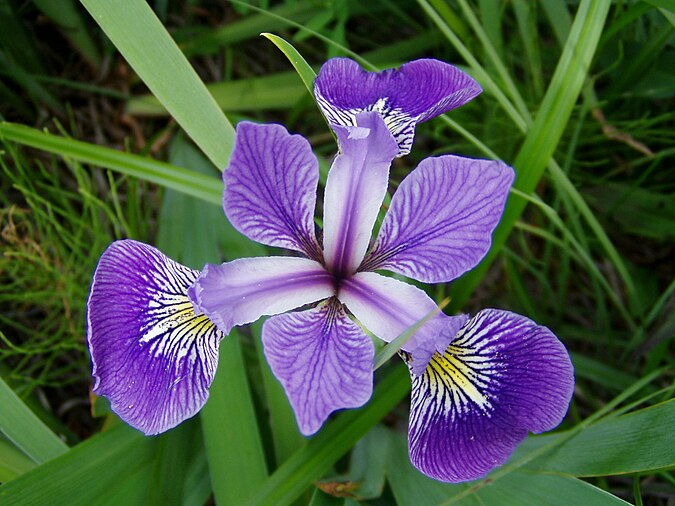
\includegraphics{2d_visualisation_files/mediabag/675px-Iris_versicolo.jpg}

}

\caption{Wiki image}

\end{figure}%

\subsection{Virginica}\label{virginica}

\begin{figure}[H]

{\centering 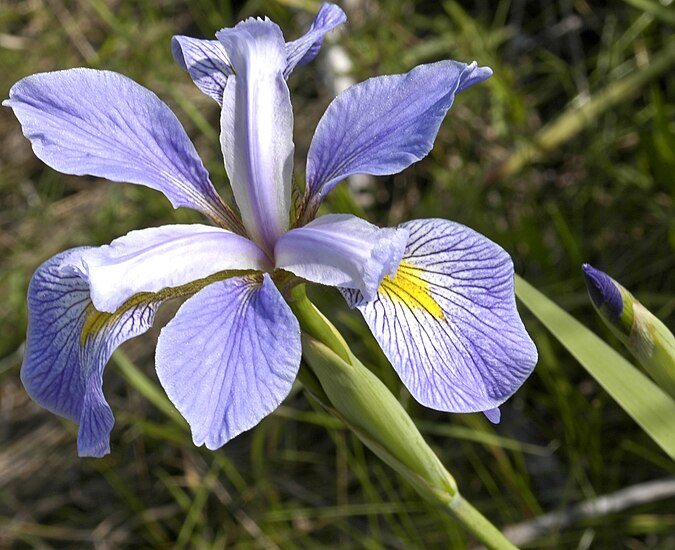
\includegraphics{2d_visualisation_files/mediabag/675px-Iris_virginica.jpg}

}

\caption{Wiki image}

\end{figure}%

\begin{center}\rule{0.5\linewidth}{0.5pt}\end{center}

\textbf{Instance:}

\begin{itemize}
\item
  150 samples/datapoints, each having over 4 numerical dimensions
  \(\mathcal{D_1,} \dots \mathcal{D_{4}}\)
\item
  an expert classification function over 3 categories
\end{itemize}

. . .

\textbf{Solution:}

a linear combination
\(\mathcal{D_1} \times \dots \mathcal{D_{4}}\rightarrow \mathcal{D_5}\)

that \emph{respects} the given classification.

. . .

\textbf{Measure:} \emph{agreement} with the given classification.

\subsection{The Iris dataset}\label{the-iris-dataset}

n=150 samples manually assigned by Fisher.

d=5 dimensions, four measurements and the classification

k=3 classes: Setosa, Versicolour and Virginica, 50 instances each, all
available from

\begin{itemize}
\item
  the \href{./data/iris.csv}{iris.csv} file from our class repo.
\item
  \href{https://scikit-learn.org/stable/auto_examples/datasets/plot_iris_dataset.html}{scikit-learn}
\item
  The \href{https://archive.ics.uci.edu/ml/datasets/iris}{UCI Machine
  Learning Repository}
\end{itemize}

\subsection{The predictors}\label{the-predictors}

\begin{itemize}
\tightlist
\item
  sepal length;
\item
  sepal width;
\item
  petal length, and
\item
  petal width.
\end{itemize}

All measurements are in cm.

\begin{center}\rule{0.5\linewidth}{0.5pt}\end{center}

\subsection{Loading the dataset}\label{loading-the-dataset}

The`\texttt{iris.csv} file is a comma separated file. To load the
dataset into the memory we follow the following steps:

\begin{enumerate}
\def\labelenumi{\arabic{enumi}.}
\tightlist
\item
  Read the file using Pandas.
\item
  For each row, split them by comma. This will create a list of strings
  for the row. Then map the strings into the float value.
\item
  Map the classes to an integer value.
\item
  Convert the row lists called as \texttt{data} in the program into a
  numpy array.
\end{enumerate}

\subsection{Histogram}\label{histogram}

A graph consisting of rectangles whose area is proportional to the
frequency of a feature and whose width is equal to the class interval
denoted as bins

\subsection{Scatter plot}\label{scatter-plot}

A scatter plot is a type of plot or mathematical diagram using Cartesian
coordinates to display values for typically two variables for a set of
data.

\begin{itemize}
\item
  A 2D visualization of datapoints against Cartesian coordinates.
\item
  Normally, the measured variable is on the x-axis.
\item
  if time is available then it is always on the x-axis.
\end{itemize}

\begin{center}\rule{0.5\linewidth}{0.5pt}\end{center}

\begin{Shaded}
\begin{Highlighting}[]
\ImportTok{from}\NormalTok{ sklearn }\ImportTok{import}\NormalTok{ datasets}
\end{Highlighting}
\end{Shaded}

\begin{Shaded}
\begin{Highlighting}[]
\NormalTok{iris }\OperatorTok{=}\NormalTok{ datasets.load\_iris()}

\BuiltInTok{print}\NormalTok{(iris[}\StringTok{\textquotesingle{}data\textquotesingle{}}\NormalTok{])}

\BuiltInTok{print}\NormalTok{(iris[}\StringTok{\textquotesingle{}target\textquotesingle{}}\NormalTok{])}
\end{Highlighting}
\end{Shaded}

\subsection{An alternative solution}\label{an-alternative-solution}

Self-study this interesting package
\href{https://pypi.org/project/ucimlrepo/}{ucimlrepo}

\begin{Shaded}
\begin{Highlighting}[]
\NormalTok{pip install ucimlrepo}
\end{Highlighting}
\end{Shaded}

\begin{Shaded}
\begin{Highlighting}[]
\ImportTok{import}\NormalTok{ pandas }\ImportTok{as}\NormalTok{ pd}
\ImportTok{from}\NormalTok{ ucimlrepo }\ImportTok{import}\NormalTok{ fetch\_ucirepo }
  
\NormalTok{ID }\OperatorTok{=} \DecValTok{53}

\NormalTok{iris }\OperatorTok{=}\NormalTok{ fetch\_ucirepo(ID) }
  
\CommentTok{\# data (as pandas dataframes) }
\NormalTok{X }\OperatorTok{=}\NormalTok{ iris.data.features }
\NormalTok{y }\OperatorTok{=}\NormalTok{ iris.data.targets }
  
\BuiltInTok{print}\NormalTok{(iris.metadata) }
  
\BuiltInTok{print}\NormalTok{(iris.variables) }
\end{Highlighting}
\end{Shaded}

\begin{center}\rule{0.5\linewidth}{0.5pt}\end{center}

\subsection{Try visualising the data}\label{try-visualising-the-data}

Open the exercise files, read the code then run it.

\begin{itemize}
\tightlist
\item
  exercise: plot the histogram of the sepal-width column
\end{itemize}

See the
\href{https://matplotlib.org/3.1.1/gallery/statistics/hist.html}{Matplotlib
tutorial}

\begin{itemize}
\tightlist
\item
  exercise: plot the scatter plot of the sepal width against the sepal
  length
\end{itemize}

See the
\href{https://matplotlib.org/3.1.1/api/_as_gen/matplotlib.pyplot.scatter.html}{Matplotlib
tutorial}

\subsection{Try at home}\label{try-at-home}

\includegraphics{./imgs/iris_all_scatterplots.png}



\end{document}
